\documentclass[a4paper,12pt]{article}
\usepackage[top = 2.5cm, bottom = 2.5cm, left = 2.5cm, right = 2.5cm]{geometry}
\usepackage[T1]{fontenc}
\usepackage[utf8]{inputenc}
\usepackage{multirow} 
\usepackage{booktabs} 
\usepackage{graphicx}
\usepackage[spanish]{babel}
\usepackage{setspace}
\setlength{\parindent}{0in}
\usepackage{float}
\usepackage{fancyhdr}
\usepackage{amsmath}
\usepackage{amssymb}
\usepackage{amsthm}
\usepackage{natbib}
\usepackage{graphicx}
\usepackage{subcaption}
\usepackage{booktabs}
\usepackage{etoolbox}
\usepackage{apalike}
\usepackage{minibox}
\usepackage{hyperref}
\usepackage{xcolor}
\usepackage{tcolorbox}
\usepackage{svg}
\usepackage{tikz}
\usepackage[framemethod=default]{mdframed}
\global\mdfdefinestyle{exampledefault}{%
linecolor=lightgray,linewidth=1pt,%
leftmargin=1cm,rightmargin=1cm,
}
\newenvironment{noter}[1]{%
\mdfsetup{%
frametitle={\tikz\node[fill=white,rectangle,inner sep=0pt,outer sep=0pt]{#1};},
frametitleaboveskip=-0.5\ht\strutbox,
frametitlealignment=\raggedright
}%
\begin{mdframed}[style=exampledefault]
}{\end{mdframed}}
\newcommand{\linea}{\noindent\rule{\textwidth}{3pt}}
\newcommand{\linita}{\noindent\rule{\textwidth}{1pt}}

\AtBeginEnvironment{align}{\setcounter{equation}{0}}
\newenvironment{solution}
  {\renewcommand\qedsymbol{$\square$}\begin{proof}[\textcolor{blue}{Solución}]}
  {\end{proof}}
\pagestyle{fancy}

\fancyhf{}
%----------------------------------------------------------
\lhead{\footnotesize Análisis de Variable Real 1}
\rhead{\footnotesize  Rudik Roberto Rompich}
\cfoot{\footnotesize \thepage}

\begin{document}
 \thispagestyle{empty} 
    \begin{tabular}{p{15.5cm}}
    \begin{tabbing}
    \textbf{Universidad del Valle de Guatemala} \\
    Departamento de Matemática\\
    Licenciatura en Matemática Aplicada\\\\
   \textbf{Estudiante:} Rudik Roberto Rompich\\
   \textbf{E-mail:} \textcolor{blue}{ \href{mailto:rom19857@uvg.edu.gt}{rom19857@uvg.edu.gt}}\\
   \textbf{Carné:} 19857
    \end{tabbing}
    \begin{center}
        MM2034 - Análisis de Variable Real 1 - Catedrático: Dorval Carías\\
        \today
    \end{center}\\
    \hline
    \\
    \end{tabular} 
    \vspace*{0.3cm} 
    \begin{center} 
    {\Large \bf  HT 5
} 
        \vspace{2mm}
    \end{center}
    \vspace{0.4cm}
%--------------------------
Las siguientes definiciones/teoremas (demostrados) fueron vistos en clase: 
\begin{tcolorbox}[colback=blue!15,colframe=blue!1!blue,title=Definición de funciones convexas]
	Sea $f : I \to \mathbb{R}$ se dice que $f$ es convexa sobre $I$, si $\forall \ s,t \in I$ y $\lambda\in [0,1]$, se tiene que: 
	$$f( \lambda s+(1 -\lambda)t) \leq \lambda f(s)+ (1 - \lambda)f(t).$$
	\begin{enumerate}
		\item $f$ es función cóncava sobre $I$ si $-f$ es convexa sobre $I$.
	\end{enumerate}
\end{tcolorbox}

\begin{tcolorbox}[colback=gray!15,colframe=gray!1!gray,title=Teorema (Desigualdad de Jensen)]
	Sea $f$ una función convexa y $w_1,w_2,\cdots, w_n$, tal que: 
	\begin{enumerate}
		\item $w_j\geq 0$.
		\item $\sum_{j=1}^{n}w_j =1$. 
	\end{enumerate}
Entonces para $x_1,x_2,\cdots, x_n$, se cumple: 
$$f\left(w_1x_1+w_2x_2+\cdots + w_nx_n\right)\leq w_1f(x_1)+\cdots +w_nf(x_n).$$
Que es igual a 
$$f\left(\sum_{j=1}^{n}w_jx_j\right)\leq \sum_{j=1}^{n}w_jf(x_j).$$
\end{tcolorbox}

\begin{tcolorbox}[colback=gray!15,colframe=gray!1!gray,title=Lema (De las tres cuerdas)]
	Sea $f:I\to\mathbb{R}$, entonces $f$ es convexa si y solo si $\forall \ x_1,x_2,x_3\in I$, $x_1<x_2<x_3$, se tiene que: 
	$$\frac{f(x_2)-f(x_1)}{x_2-x_1}\leq \frac{f(x_3)-f(x_1)}{x_3-x_1}\leq \frac{f(x_3)-f(x_2)}{x_3-x_2}.$$
\end{tcolorbox}




\section{Problema 1}
\begin{tcolorbox}[colback=blue!15,colframe=blue!1!blue,title=Definición del valor intermedio]
Si $f(a)<c<f(b)$, entonces $f(x)=c$ para algún $x$ entre $a$ y $b$. 
\end{tcolorbox}


\begin{tcolorbox}[colback=gray!15,colframe=gray!1!gray,title=Teorema 1 (Demostrado en clase)]
La imagen de un compacto bajo un mapeo continuo es compacto.
\end{tcolorbox}
\begin{tcolorbox}[colback=blue!15,colframe=blue!1!blue,title=Definición de punto límite de \cite{rudin1976principles}]
	Si $p$ es un punto límite de un conjunto $E$, entonces cada vecindad de $p$ contiene infinitos puntos contables de $E$. 
\end{tcolorbox}

\begin{tcolorbox}[colback=gray!15,colframe=gray!1!gray,title=Caracterización secuencial de compacto (Demostrado en clase)]
	Un subconjunto $K$ de $\mathbb{R}$ es compacto si y solo si cada sucesión en $K$ tiene una subsucesión que converge a un punto en $K$.
\end{tcolorbox}

Demuestre que la función $f: \mathbb{R} \to \mathbb{R}$ es continua ssi $f$ tiene la propiedad del valor intermedio y mapea conjuntos compactos en conjuntos compactos.

\begin{proof}
	Nótese que es una prueba de ida y de vuelta.
	\begin{enumerate}
		\item[\fbox{$\to$}] A probar: $f$ tiene la propiedad del valor intermedio y mapea conjuntos compactos en conjuntos compactos. Por hipótesis sabemos que $f$ es continua, entonces por el teorema del valor intermedio de Bolzano $f$ debe tener la propiedad del valor intermedio.  $$\implies \exists \ c \in \mathbb{R} \ni f(c)=k, \quad k \in \mathbb{R}.$$
		Por lo tanto, por la caracterización secuencial de compactos, nos garantiza que el subconjunto que mapea la función es compacto en un intervalo $[a,b]$ si cada sucesión en el subconjunto  tiene una subsucesión que converge a algún punto en el subconjunto (a mayor detalle en la prueba de regreso). Además,  por el teorema 1, la compacidad de conjuntos compactos se preserva bajo un mapeo continuo. 
		
		\item [\fbox{$\gets$}] Por contradicción. Sea asume que $f$ no es continua. Además, tenemos:
		\begin{enumerate}
			\item Una función mapea conjuntos compactos en conjuntos compactos. Además, nótese que por Heine-Borel, un conjunto compacto es cerrado y acotado. Entonces, tenemos una función $f$ que mapea $[a,b]\to [a,b]$.
			\item  Considérese la caracterización secuencial del compacto. Entonces dígase que si $x_n\to x_0$. Pero ahora, nótese que nos dicen que $f$ tiene la propiedad del valor intermedio tal que: 
			$$f(x_0)<c<f(x_n), \qquad \ c\in [a,b] \text{ y } \forall \ n.$$ 
			Entonces, $f(z_n)=c$, en donde $z_n\in (x_0, x_n)$. Por lo que podemos asumir que, $z_n \to x_0$. Ahora, notamos que $x_0$ debe ser un \textbf{punto límite} del conjunto $z$, tal que $f(z)=c$; sin embargo, por el inciso \textbf{a} sabemos que $[a,b]$ es cerrado, pero $z$ no pertenece al conjunto $x_0$. ($\to\gets$) Entonces $f$ debe ser continua.
		\end{enumerate}
		
	\end{enumerate}
\end{proof}

\section{Problema 2}
\begin{tcolorbox}[colback=gray!15,colframe=gray!1!gray,title= Propiedad 1 ]
	Sea $I$ un intervalo  y $f:I\to \mathbb{R}$ una función convexa. Para cada $a\in I$. Considere $f_a: I-\{a\}\to \mathbb{R}\ni $: 
	$$f_a(x)=\frac{f(x)-f(a)}{x-a}.$$
	Entonces, $f_a(x)$ es creciente en $I$. 
\end{tcolorbox}
Sea $I$ un intervalo y $f$ una función con primera derivada continua en $I$, los enunciados siguientes son equivalentes. 
\begin{noter} {Nota}
	(3)$\implies$ (1) $\iff$ (2). $\therefore (3) \implies (2)$.
\end{noter}
\begin{enumerate}
	\item $f$ es convexa. 
	\begin{proof}
		(1)$\implies$ (2). Por hipótesis sabemos que $f:I\to\mathbb{R}$ es convexa y es diferenciable. Por la \textbf{propiedad 1} (demostrada en clase), $\forall \ x_1,x_2,x_3,x_4\in I$, $x_1<x_2<x_3<x_4$, se tiene que: 
		$$\frac{f(x_2)-f(x_1)}{x_2-x_1}\leq \frac{f(x_3)-f(x_2)}{x_3-x_2}\leq \frac{f(x_4)-f(x_3)}{x_4-x_3} .$$
		Es decir
		$$\frac{f(x_2)-f(x_1)}{x_2-x_1}\leq\frac{f(x_4)-f(x_3)}{x_4-x_3}.$$
		Ahora bien, como sabemos que $f$ es diferenciable, consideremos la definición de derivada lateral $\ \ni $
		$$\lim_{x_2\to x_1^+}\frac{f(x_2)-f(x_1)}{x_2-x_1}\leq\lim_{x_3\to x_4^-}\frac{f(x_4)-f(x_3)}{x_4-x_3}\implies f'(x_1)\leq f'(x_4).$$
		$\therefore \ f'$ es creciente. 
	\end{proof}






	\item $f'$ es creciente. 
		\begin{proof}
		(2)$\implies$ (1). Por hipótesis sabemos que $f'$ es creciente. Supóngase  $\forall x_1,x_2,x_2\in I$, $x_1<x_2<x_3$. Se tiene por el \textbf{teorema del valor medio} de \cite{bartle2000introduction}, $\exists \ u, v \ \ni u\in (x_1,x_2)$ y $v\in (x_2,x_3)$; entonces: 
		$$f'(u)=\frac{f(x_2)-f(x_1)}{x_2-x_1}\qquad \text{y } \qquad f'(v)=\frac{f(x_3)-f(x_2)}{x_3-x_2} $$   
		Como sabíamos que $f'$ es creciente, entonces: 
		$$f'(u)\leq f'(v)\implies \frac{f(x_2)-f(x_1)}{x_2-x_1} \leq\frac{f(x_3)-f(x_2)}{x_3-x_2} .$$
		$\therefore \ f$ es convexa por la \textbf{propiedad 1} (demostrada en clase).  
	\end{proof}




	\item $\forall \ a,x  \in I$, se tiene $f(x)\geq f(a)+f'(a)(x-a)$.
		\begin{proof}
		(3)$\implies$ (1). A probar que $f$ es una función convexa. Se propone tratar el problema con dos casos distintos para $x$.  Sean $s,t\in I $ y $\lambda\in [0,1]$, además $a:=\lambda y+ (1-\lambda)x$, es decir: 
		
		\begin{enumerate}
			\item Caso 1. 
			$$f(s)\geq f(a)+f'(a)(s-a), \qquad a:= \lambda s+(1-\lambda)t.$$
			Entonces:
			\begin{align*}
				f(s) &\geq f(a)+f'(a)(s-a)\\
				       &\geq f(\lambda s+(1-\lambda)t)+f'(\lambda s+(1-\lambda)t)(s-( \lambda s+(1-\lambda)t))\\
				       &\geq f(\lambda s+(1-\lambda)t)+f'(\lambda s+(1-\lambda)t)(s-( \lambda s+t-\lambda t))\\
				       &\geq  f(\lambda s+(1-\lambda)t)+f'(\lambda s+(1-\lambda)t)(s- \lambda s -t+\lambda t)\\
				       &\geq  f(\lambda s+(1-\lambda)t)+f'(\lambda s+(1-\lambda)t)(s-t)(1-\lambda)\\
				       &\geq  f(\lambda s+(1-\lambda)t)-f'(\lambda s+(1-\lambda)t)(t-s)(1-\lambda)
				       \intertext{Ahora, multiplicando por $\lambda$. }
				    \lambda f(s)  &\geq  \lambda \left[f(\lambda s+(1-\lambda)t)-f'(\lambda s+(1-\lambda)t)(t-s)(1-\lambda)\right].
			\end{align*}
			\item Caso 2. 
			$$f(t)\geq f(a)+f'(a)(t-a), \qquad a:= \lambda s+(1-\lambda)t.$$
			Entonces: 
			\begin{align*}
				f(t) &\geq f(a)+f'(a)(t-a)\\
				&\geq f(\lambda s+(1-\lambda)t)+f'(\lambda s+(1-\lambda)t)(t-( \lambda s+(1-\lambda)t))\\
				&\geq f(\lambda s+(1-\lambda)t)+f'(\lambda s+(1-\lambda)t)(t-\lambda s-t+\lambda t)\\
				&\geq f(\lambda s+(1-\lambda)t)+f'(\lambda s+(1-\lambda)t)\lambda (t-s)
				\intertext{Ahora, multiplicando por $(1-\lambda)$. }
					(1-\lambda)f(t) &\geq (1-\lambda) \left[f(\lambda s+(1-\lambda)t)+f'(\lambda s+(1-\lambda)t)\lambda (t-s)\right].
			\end{align*}
		Si sumamos las desigualdades de ambos casos, tenemos: 
		$$\lambda f(s)  +	(1-\lambda)f(t) \geq f( \lambda s+(1 -\lambda)t).$$
		Por lo tanto, $f$ es convexa.
		\end{enumerate}

	\end{proof}
\end{enumerate}
\section{Problema 3}
\begin{tcolorbox}[colback=gray!15,colframe=gray!1!gray,title=Teorema caracterización monótono (demostrado en clase)]
	Suponga que $f:(a, b) \rightarrow \mathbb{R}$ es diferenciable sobre $(a, b)$. Entonces,\newline
	(1) $f$ es creciente ssi $f^{\prime}(x) \geqslant 0$, $\quad  \forall x \in(a, b)$.\newline
	(2) $f$ es decreciente ssi $f^{\prime}(x) \leqslant 0, \quad \forall x \in(a, b)$
\end{tcolorbox}
\begin{noter}{Teorema importante}
	Para resolver los siguientes problemas que se presentan, primero se demostrará \textit{con un método alternativo} el siguiente teorema de \cite{bartle2000introduction}. 
	\begin{tcolorbox}[colback=gray!15,colframe=gray!1!gray,title=Teorema  6.4.6]
		Let $I$ be an open interval and let $f : I \to \mathbb{R}$ have a second derivative on $I$. Then $f$ is a convex function on $I$ if and only if $f''(x)\geq 0$ for all $x \in I$.
	\end{tcolorbox}


\begin{proof}
	Es un teorema de caracterización, por lo cual: 
	\begin{enumerate}
		\item $(\to)$ Trivial. Por el teorema resuelto en el \textbf{Problema 1}, sabemos que $f'$ es creciente. Ahora bien, por el teorema de caracterización monótono (demostrado en clase) sabemos que $f''(x)\geq 0$. 
		\item $(\gets)$ Se tomará en cuenta la idea de \cite{tiel1984convex}. 
		Sea $x, y \in I, x<y$ y $\lambda\in (0,1)$. Por \textbf{teorema del valor medio} de \cite{bartle2000introduction}, sabemos que existe\newline $$\xi_{1}, \xi_{2}, x<\xi_{1}<\lambda x+(1-\lambda) y<\xi_{2}<y$$y  $$\xi_{3}, \xi_{1}<\xi_{3}<\xi_{2}$$
		tal que
		$$
		\begin{aligned}
			f(\lambda&x+(1-\lambda) y)-\lambda f(x)-(1-\lambda) f(y) \\
			&=\lambda[f(\lambda x+(1-\lambda) y)-f(x)]+(1-\lambda)[f(\lambda x+(1-\lambda) y)-f(y)] \\
			&=\lambda(1-\lambda)(y-x) f^{\prime}\left(\xi_{1}\right)+(1-\lambda) \lambda(x-y) f^{\prime}\left(\xi_{2}\right) \\
			&=\lambda(1-\lambda)(y-x)\left(\xi_{1}-\xi_{2}\right) f^{\prime \prime}\left(\xi_{3}\right) \leqslant 0 .
		\end{aligned}
		$$
		Por lo tanto $f$ es convexo.
	\end{enumerate}
\end{proof}
\end{noter}
Compruebe que la función: 
\begin{enumerate}
	\item $f(x)=e^x$ es convexa. 
	\begin{figure}[ht]
		\centering
		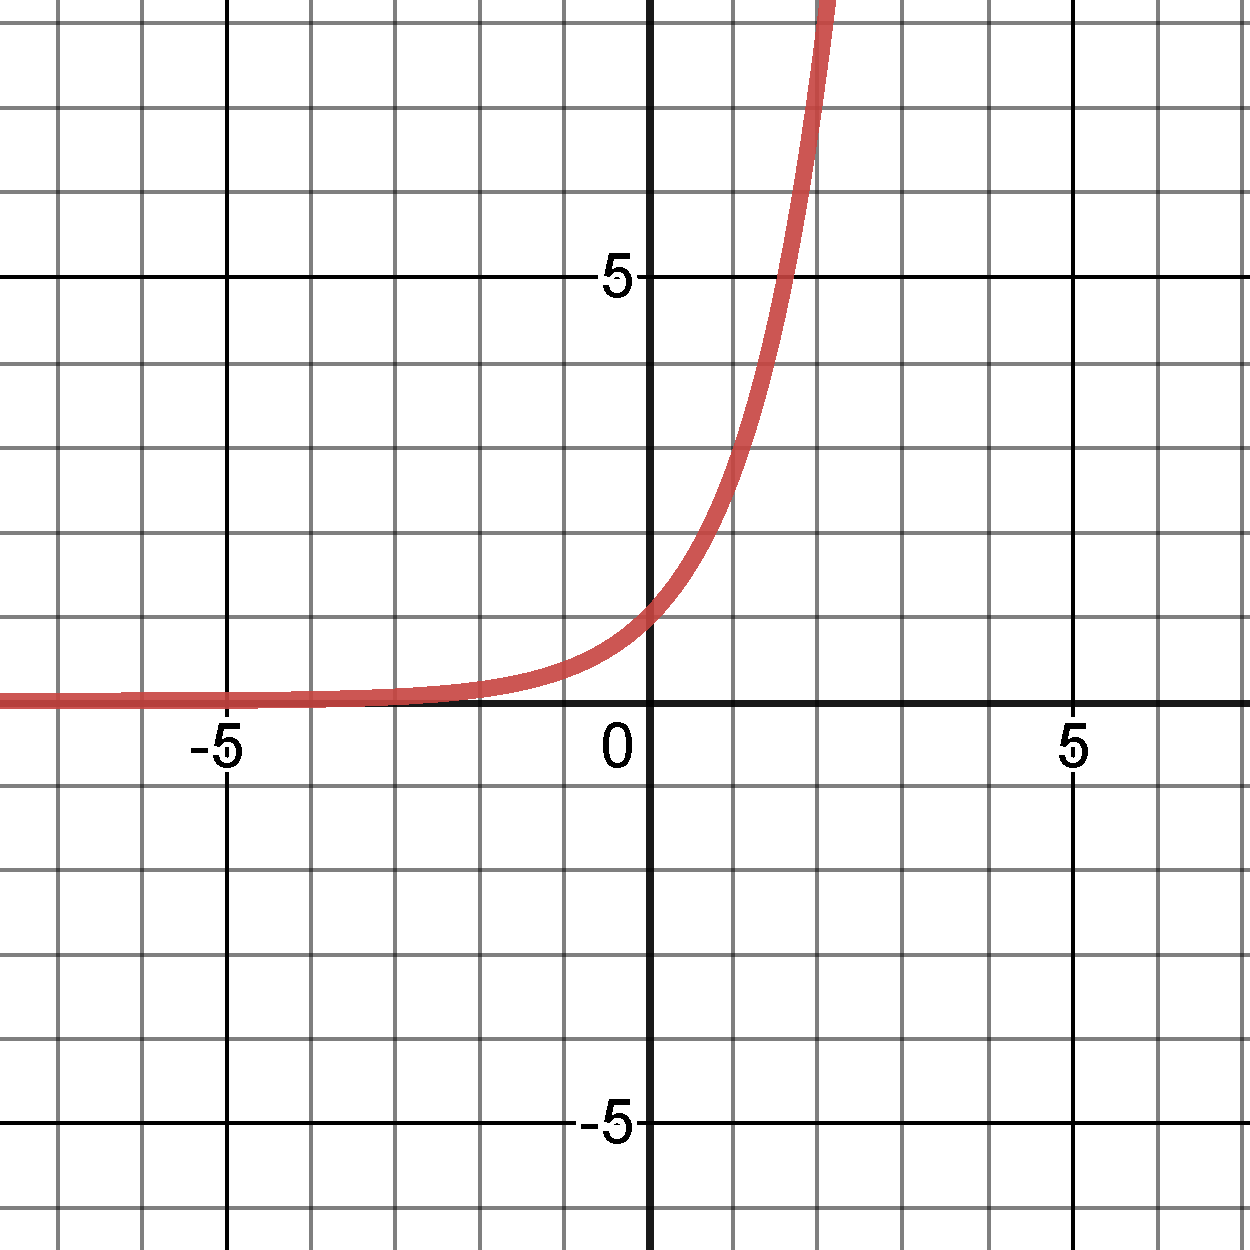
\includegraphics[scale=0.3]{/Users/rudiks/Git/Real_Analysis/HT5/Imagenes/1.pdf}
		\caption{$f(x)=e^x$}
	\end{figure}

		\begin{proof}
		Por el \textbf{teorema importante}, entonces se tiene: 
		$$\implies f(x)=e^x \implies f'(x) =e^x \implies f''(x)= e^x.$$
		Entonces, $f''(x)\geq 0$. Por lo tanto, es una función convexa.
	\end{proof}


%--------------------------

	\item $f(x)=\ln x$ es cóncava. 
		\begin{figure}[ht]
		\centering
		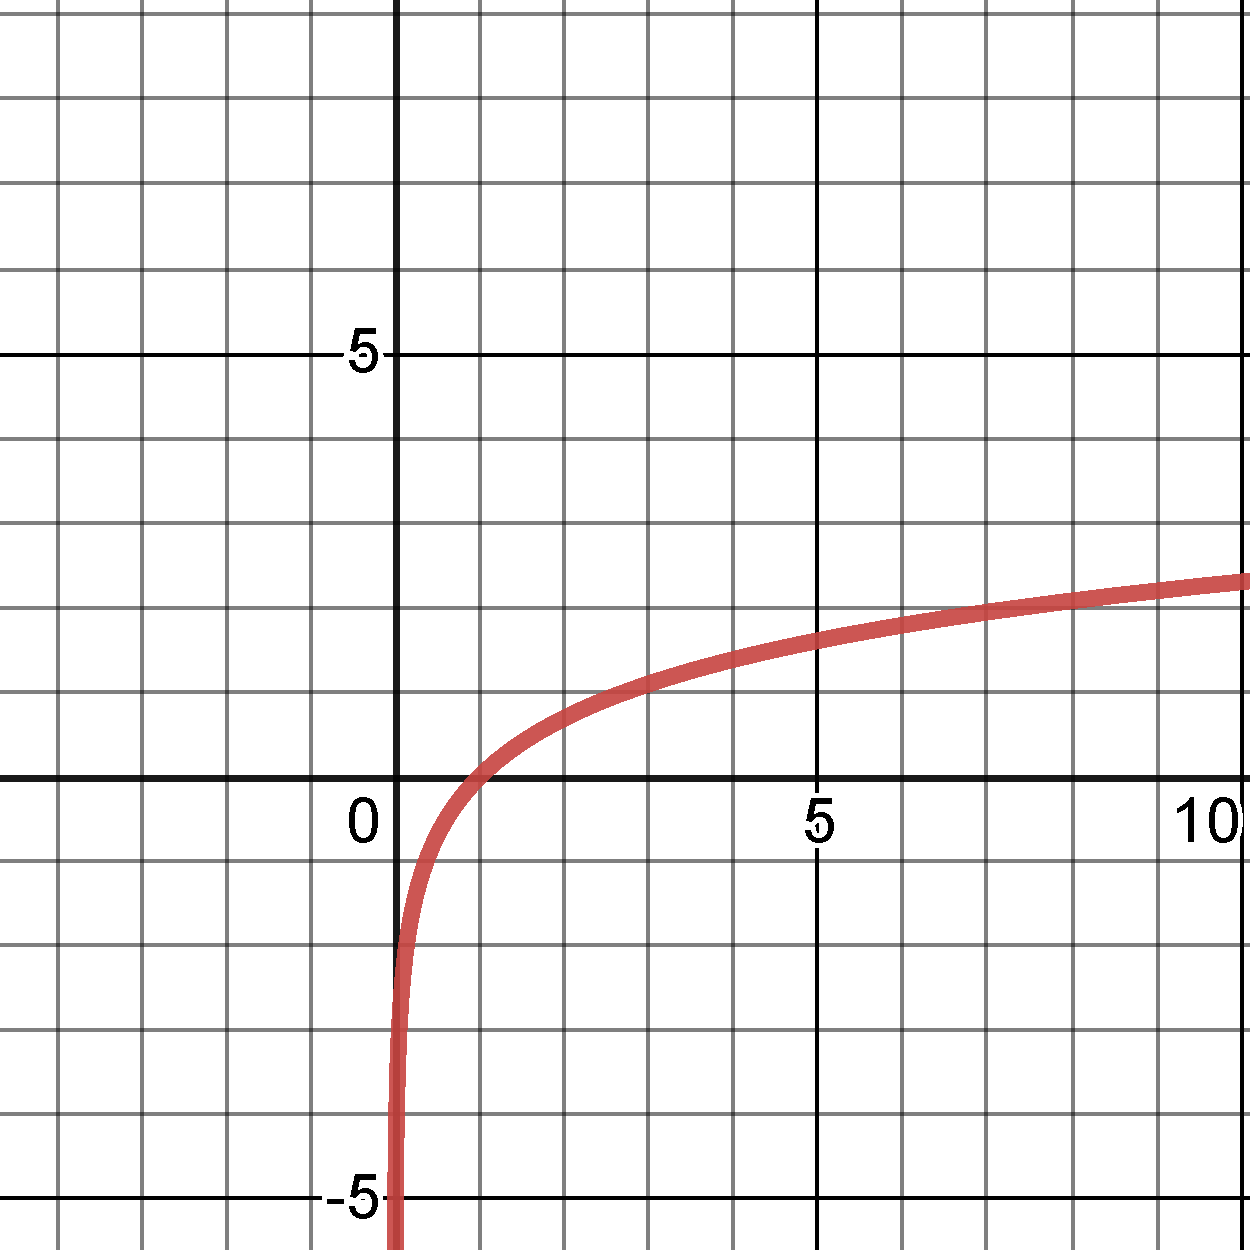
\includegraphics[scale=0.3]{/Users/rudiks/Git/Real_Analysis/HT5/Imagenes/2.pdf}
		\caption{$f(x)=\ln x$}
	\end{figure}
		\begin{proof}
		Por la definición de cóncavo, se probará: $f(x)=-\ln x$ es convexa. Por el \textbf{teorema importante}:
		$$\implies f(x)=-\ln x\implies f'(x)=-\frac{1}{x}\implies f''(x)=\frac{1}{x^2}.$$
		Entonces, $f''(x)\geq 0$. Por lo tanto, es una función convexa. Por la definición, entonces $f(x)=\ln x$ es cóncava. 
	\end{proof}


%--------------------------





	\item $f(x)=x^\alpha$, es $\begin{cases}
		\text{Convexa, si} & \alpha \leq 0 \text{ o } \alpha \geq 1\\
		\text{Cóncava, si} & 0 \leq \alpha \leq 1
	\end{cases}$
\begin{figure}[ht]
	\begin{tabular}{cc}
		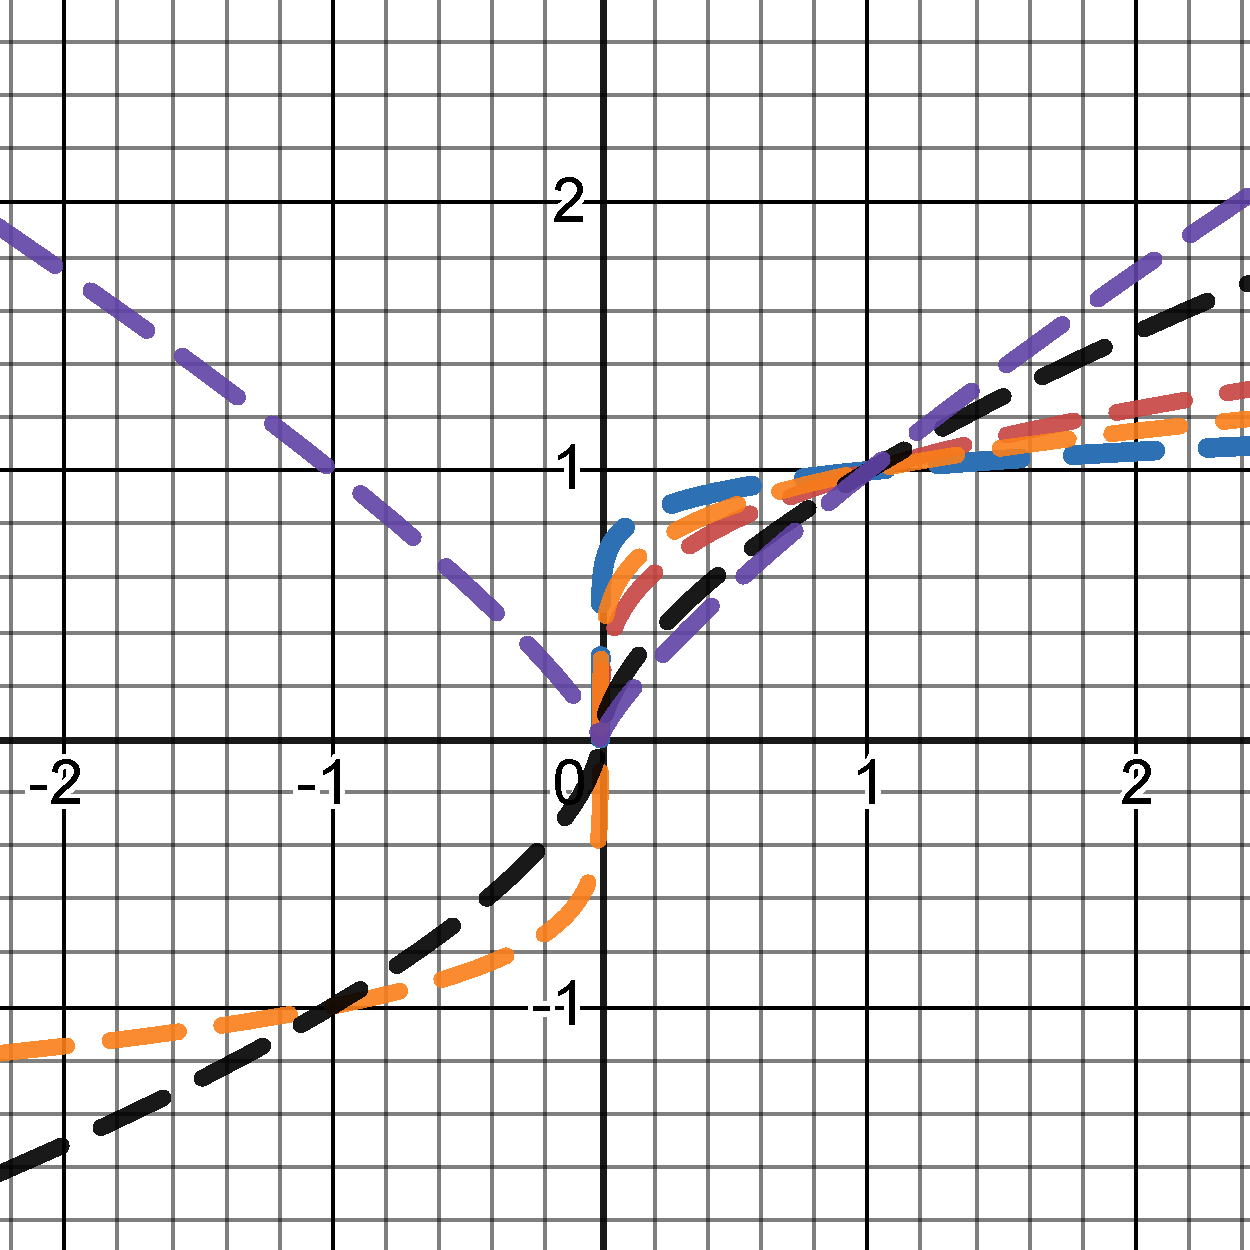
\includegraphics[width=65mm]{/Users/rudiks/Git/Real_Analysis/HT5/Imagenes/3.1.pdf} &   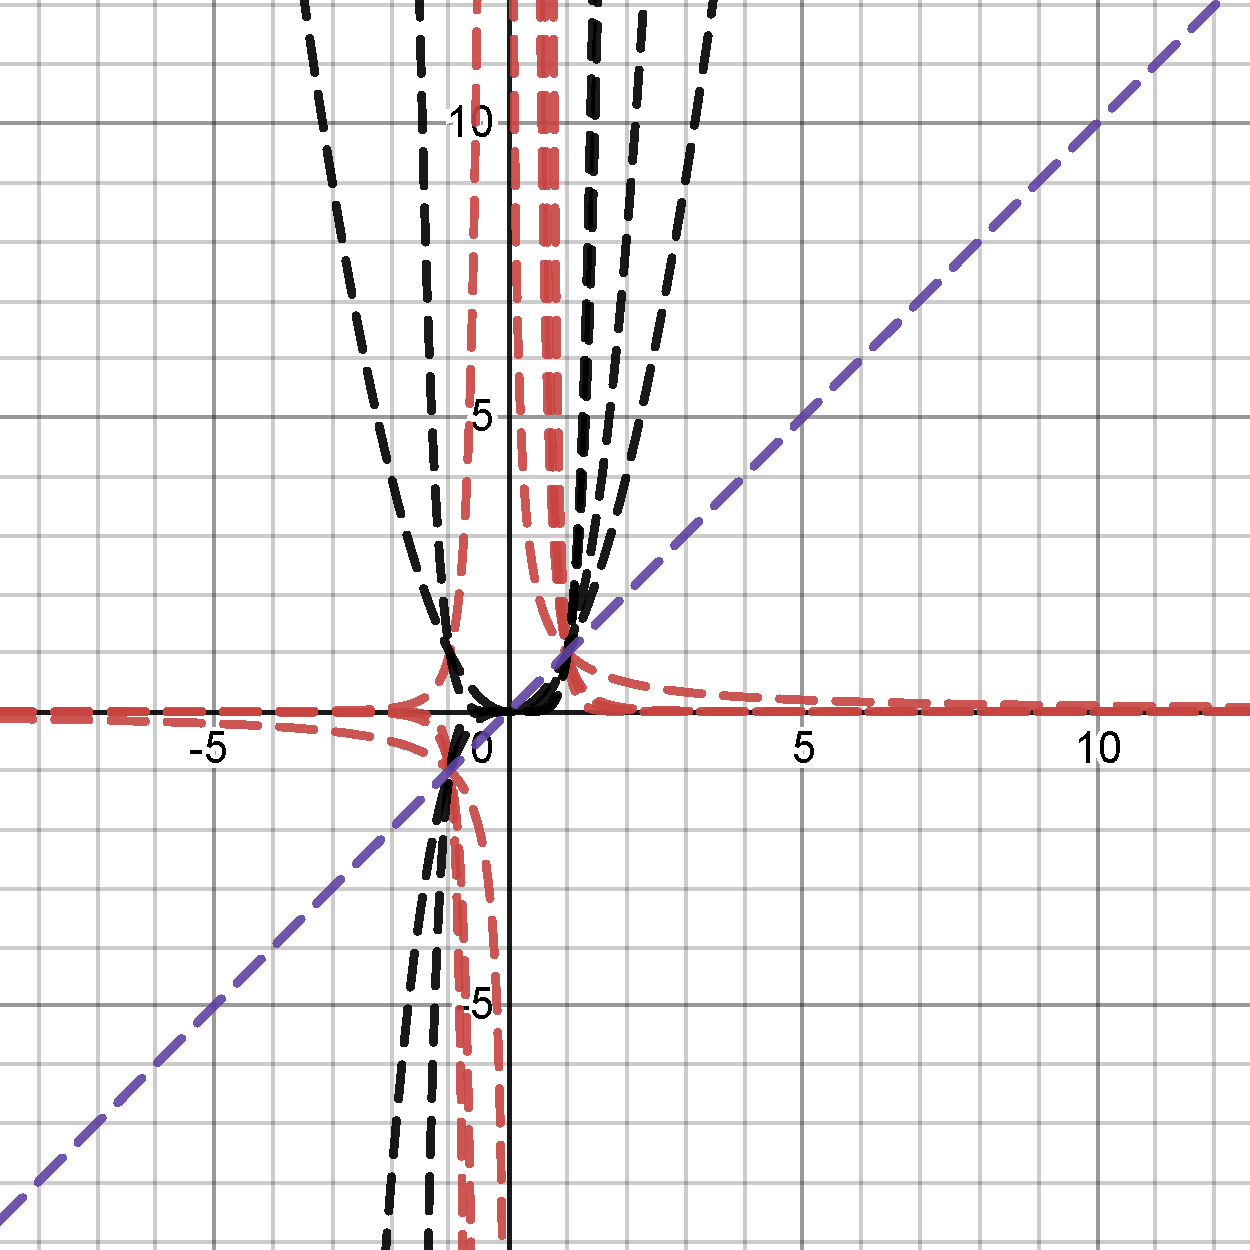
\includegraphics[width=65mm]{/Users/rudiks/Git/Real_Analysis/HT5/Imagenes/3.2.pdf} \\
		(a) $\alpha \leq 0 \text{ o } \alpha \geq 1$ & (b) $0 \leq \alpha \leq 1$
	\end{tabular}
	\caption{$f(x)=x^\alpha$}
\end{figure}
	\begin{proof}Comenzamos calculando la segunda derivada: 
		\begin{gather}
			\implies f(x)=x^\alpha \implies f'(x)=\alpha x^{\alpha -1}\implies f''(x)=\alpha (\alpha -1)x^{\alpha -2}.
		\end{gather}
	Análogamente: 
	\begin{gather}
		\implies f(x)=-x^\alpha \implies f'(x)=-\alpha x^{\alpha -1}\implies f''(x)=-\alpha (\alpha -1)x^{\alpha -2}.
	\end{gather}
	Nótese que tenemos dos casos:
	\begin{enumerate}
		\item $f(x)=x^\alpha$ es convexa, $\alpha \leq 0$ o $\alpha \geq 1$. Es decir, tenemos: $$\alpha \in (-\infty, 0] \qquad \text{ o }\qquad  \alpha \in [1,\infty).$$
		Considérese la segunda derivada obtenida en (1), por el \textbf{teorema importante} la condición se cumple trivialmente para $\alpha \in (-\infty,0]\cup [1,\infty)$; ya que $f''(x)\geq 0$ en todos los casos. Por lo tanto es convexa.
		\item $f(x)=x^\alpha$ es cóncava, $0\leq \alpha \leq 1$. Es decir, tenemos:
		$$a\in [0,1].$$
			Por la definición de cóncavo, se probará $x^\alpha$ es convexa. Considérese la segunda derivada de $f(x)=-x^{\alpha}$ obtenida en (3), por el \textbf{teorema importante} la condición se cumple trivialmente para $\alpha \in [0,1]$; ya que $f''(x)\geq 0$ en todos los casos. Por lo tanto es convexa y por la definición de función cóncava, $x^\alpha$ es cóncava en $a\in [0,1]$.
	\end{enumerate}
\end{proof}
\end{enumerate}
%---------------------------
\bibliographystyle{apalike}
\bibliography{sample.bib}

\end{document}